\section{十二}

\subsection{十二因缘}
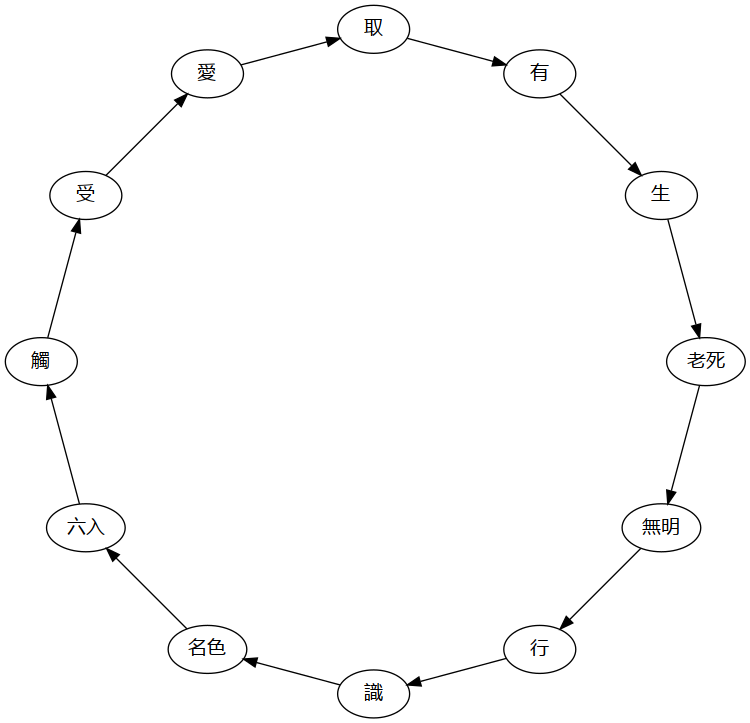
\includegraphics[scale=0.5]{释家/images/十二因缘.png}
苦、集二諦的解釋,是緣生法,也就是十二因緣\footnote{說明人生的由來和生命的流轉,自前生、今生而到後生之間的因果關係,即稱為三世兩重因果}法。
\begin{itemize}
  \item 無明:即是無智慧,是貪欲、瞋恨、愚癡等的煩惱,也是種種蠢動心理的迷惑之源。
  \item 行:即是前生造作的善惡諸業─身心的行為。
  \item 識:即是由過去世的業力,感受果報之初起妄念而托母胎,投為今生的神識。
  \item 名色:即是入胎後胎兒的身心狀態。
  \item 六入:即是在胎中長成的眼、耳、鼻、舌、身、意等六種感覺器官─六根。
  \item 觸:即是出胎後,自己的六根與外在的色、聲、香、味、觸、法等六塵相對接觸。
  \item 受:即是由接觸外境所感知的苦及樂的心境。
  \item 愛:即是厭苦欣樂而貪染財、色、名、食、睡等五欲的心理活動。
  \item 取:即是因欲愛旺盛而對於貪染諸境起取著心。
  \item 有:即是由於今生造作了有漏之因,而導致感受未來世的生死之果。
  \item 生:即是因了今生造作的業種,所感受來生的色、受、想、行、識的五蘊之身。
  \item 老死:來生既有了五蘊假合之身的出生,必將衰老而至死亡。
\end{itemize}
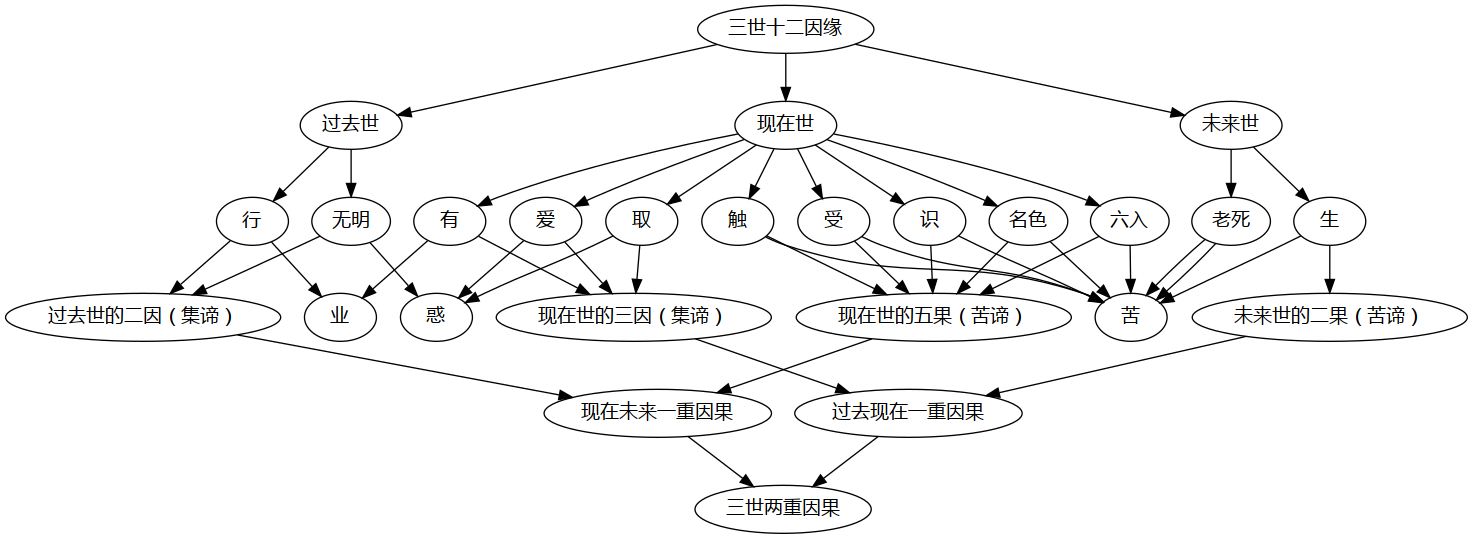
\includegraphics[scale=0.3]{释家/images/三世十二因缘.png}
\begin{table}[H]
  \centering
  \small
  \caption[]{三世十二因缘}
  \begin{tabular}{|c|c|c|c|c|c|c|c|c|c|c|c|}
    \hline \multicolumn{2}{|c}{未来世} & \multicolumn{8}{|c}{现在世} & \multicolumn{2}{|c|}{过去世} \\
    \hline 老死 & 生 & 有 & 取 & 爱 & 受 & 触 & 六入 & 名色 & 识 & 行 & 无明 \\
    \hline \multicolumn{2}{|c|}{苦} & 业 & \multicolumn{2}{c|}{惑} & \multicolumn{5}{c|}{苦} & 业 & 惑 \\
    \hline \multicolumn{2}{|c}{未来世的二果(苦谛)} & \multicolumn{3}{|c}{现在世的三因(集谛)} & \multicolumn{5}{|c}{现在世的五果(苦谛)} & \multicolumn{2}{|c|}{过去世的二因(集谛)} \\
    \hline \multicolumn{5}{|c|}{现在未来一重因果} & \multicolumn{7}{c|}{过去现在一重因果} \\
    \hline \multicolumn{12}{|c|}{三世两重因果} \\
    \hline
  \end{tabular}
\end{table}
